\documentclass[11pt]{article}

\usepackage[utf8]{inputenc}
\usepackage[T1]{fontenc}
\usepackage{lmodern}
\usepackage[a4paper,margin=2.5cm]{geometry}
\usepackage{setspace}
\usepackage{graphicx}
\usepackage{booktabs}
\usepackage{amsmath,amssymb}
\usepackage{hyperref}
\usepackage{xcolor}
\usepackage{enumitem}
\usepackage{caption}
\usepackage{subcaption}
\usepackage{pgfplots}

\pgfplotsset{compat=1.18}

\hypersetup{
    colorlinks=true,
    linkcolor=blue,
    citecolor=blue,
    urlcolor=blue
}

\title{Offline Generation of Dynamic Areas of Interest for 360\textdegree\ Video in Virtual Reality with Eye Tracking: Validation Against Manual Annotations and Downstream Gaze Metrics}
\author{}
\date{}

\begin{document}

\maketitle

\begin{abstract}
This paper presents a methodological pipeline for the offline generation of dynamic areas of interest (AOIs) in 360\textdegree\ video, integrated with eye tracking in virtual reality. Rather than framing the contribution as a software integration alone, we evaluate whether automatically generated AOIs preserve downstream gaze-based metrics relative to manually annotated AOIs. The system combines frame-synchronised gaze logging, spherical gaze-to-video mapping, and per-frame AOI lookup in Unity, while AOIs are constructed offline to preserve runtime determinism and experimental traceability. We define the system architecture, describe the validation framework, and compare automatic and manual AOIs both spatially and in terms of downstream eye-tracking metrics. Results are intended to determine the extent to which annotation effort can be reduced without compromising experimental validity.
\end{abstract}


\section{Introduction}

Dynamic area-of-interest (AOI) analysis in immersive 360$^{\circ}$ video remains methodologically demanding. Unlike conventional 2D stimuli, 360$^{\circ}$ equirectangular video introduces domain-specific difficulties that directly affect both AOI construction and gaze interpretation, including seam discontinuities, projection distortion, temporal drift in dynamic objects, and the substantial burden associated with frame-by-frame manual annotation. At the same time, recent virtual reality hardware makes eye tracking increasingly accessible in head-mounted displays, creating an opportunity to develop reproducible pipelines that connect gaze acquisition, dynamic AOI assignment, and downstream metric extraction in immersive environments.

The central challenge is not merely to build a functional system, but to establish whether automatically generated dynamic AOIs remain valid for experimental gaze analysis. In this context, a purely engineering-oriented contribution would be insufficient. The key methodological question is whether AOIs generated offline can preserve the interpretability of gaze--AOI measures relative to manually annotated AOIs while reducing annotation effort and maintaining traceability of the experimental pipeline.

This work addresses that problem through an architecture that deliberately separates offline AOI construction from runtime experimental execution. In the proposed approach, artificial intelligence is used outside the Unity runtime to detect, segment, and temporally propagate AOIs over 360$^{\circ}$ video, whereas the experimental runtime remains lightweight and deterministic, being limited to stimulus presentation, frame-synchronised gaze acquisition, spherical gaze mapping, AOI lookup, and logging. This design is intended to reduce latency, simplify debugging, facilitate methodological auditing, and prevent the variability of computer-vision models from affecting real-time experimental behaviour.

The contribution of this paper is therefore methodological rather than merely instrumental. Specifically, we propose an offline pipeline for dynamic AOI generation in 360$^{\circ}$ video integrated with eye tracking in virtual reality, and we evaluate the extent to which automatically generated AOIs preserve gaze-based metrics with respect to manually annotated AOIs. The paper is not centred on real-time inference inside the engine, nor on the simple integration of existing models. Instead, it focuses on experimental validity, reproducibility, and annotation-effort reduction.

The study is guided by the following research questions:

\begin{itemize}
    \item \textbf{RQ1.} To what extent do automatically generated dynamic AOIs in 360$^{\circ}$ video preserve gaze-based metrics when compared with manually annotated AOIs?
    \item \textbf{RQ2.} Which 360$^{\circ}$-specific conditions most degrade the performance of automatic AOIs, particularly seam crossings, equirectangular distortion, small objects, and temporal drift?
    \item \textbf{RQ3.} How much annotation effort can be reduced by the proposed offline AOI pipeline while maintaining acceptable experimental validity?
\end{itemize}

From these questions, the following hypotheses are derived:

\begin{itemize}
    \item \textbf{H1.} Automatically generated AOIs will achieve sufficient spatial agreement with manually annotated AOIs to support downstream gaze analysis.
    \item \textbf{H2.} Downstream gaze metrics computed from automatic AOIs will show limited degradation relative to those computed from manual AOIs.
    \item \textbf{H3.} The offline AOI pipeline will substantially reduce annotation effort compared with manual frame-by-frame annotation.
    \item \textbf{H4.} Performance degradation will be concentrated in known 360$^{\circ}$ failure cases, especially seam discontinuities, highly distorted regions, temporally unstable objects, and small targets.
\end{itemize}

In line with these objectives, the paper focuses on five primary families of outcome measures: spatial agreement between manual and automatic AOIs, frame-synchronised technical performance of the runtime, downstream gaze-based metrics such as time to first fixation and fixation duration, exclusion and validity indicators for eye-tracking quality, and comparative annotation cost. This combination allows the proposed system to be evaluated not only as a visual-computing pipeline, but also as a measurement instrument for immersive eye-tracking research.

Accordingly, the main contribution claimed in this paper can be stated as follows: \emph{an offline pipeline for dynamic AOI generation in 360$^{\circ}$ video, integrated with virtual-reality eye tracking, whose value is assessed through both spatial validation and downstream validation of gaze--AOI metrics against a manual ground truth}. By positioning the work in these terms, the study aims to contribute a reproducible methodological framework for immersive gaze analysis rather than a software prototype alone.

\section{Related Work}

The present work sits at the intersection of four lines of research and practice: dynamic AOI analysis in moving stimuli, eye tracking in immersive virtual reality, 360$^{\circ}$ video as a spherical stimulus domain, and offline computer-vision pipelines for object-conditioned annotation. In all four areas, the central methodological issue is not only whether a technical pipeline can be made to work, but whether the resulting representations remain valid for later interpretation.

First, dynamic AOIs differ from static screen-based AOIs because the annotated target may move, deform, disappear, reappear, or become partially occluded. For conventional 2D stimuli, manual frame-by-frame annotation is already labour intensive; for immersive 360$^{\circ}$ video, the burden is compounded by seam discontinuities, projection distortion, and the need to reason in a spherical rather than planar viewing space. This makes the annotation bottleneck one of the main obstacles to scaling gaze studies in realistic immersive stimuli.

Second, virtual-reality eye tracking introduces its own experimental constraints. Head-mounted displays provide access to gaze direction within a moving head-centred reference frame, but experimental validity depends on calibration quality, tracking loss handling, runtime latency, and consistent synchronisation between displayed frames and gaze samples. In practical terms, modern OpenXR runtimes and vendor extensions make such access increasingly feasible \cite{openxr_eye_gaze_ext,vive_openxr_overview,vive_eye_gaze,vive_eye_tracker}, but methodological care is still required to turn device-level data into auditable experimental measures.

Third, 360$^{\circ}$ video is not merely ``a wide video''. Equirectangular projection introduces unequal spatial distortion across latitude, while the left-right seam can split a single object into two disconnected image regions. As a consequence, AOI definitions that seem trivial in planar video may become ambiguous near poles and seams. Runtime playback solutions in Unity also impose practical constraints on how panoramic stimuli are rendered and sampled \cite{unity_panoramic_intro,unity_panoramic_video,unity_panoramic_skybox}.

Fourth, automatic or semi-automatic AOI generation increasingly benefits from modern prompt-based detection and segmentation stacks. In principle, offline model combinations such as detector-plus-segmenter pipelines can reduce annotation cost substantially, and projects such as Grounded-SAM-2 illustrate the broader direction of this ecosystem \cite{grounded_sam2}. However, a research pipeline for immersive eye tracking requires more than visual plausibility: it requires stable instance identities, deterministic handoff to the runtime, and validation against a manual reference set.

The present draft therefore positions itself less as a generic review article and more as a system-and-methods paper. A fuller citation-backed synthesis of peer-reviewed literature on dynamic AOIs, immersive gaze analysis, and automatic annotation will be expanded in the final version. For the current implementation stage, the most relevant gap is clear: few practical pipelines explicitly connect offline dynamic AOI generation, deterministic 360$^{\circ}$ runtime playback, and downstream validation of gaze metrics under a single reproducible experimental contract.

\section{System Architecture}

The proposed system is structured into three layers: offline AOI construction, runtime experimental execution in Unity, and post hoc analysis of gaze-AOI metrics.

\subsection{Offline AOI generation}
AOIs are generated offline in order to keep the runtime lightweight, deterministic, and auditable. In the current implementation, this layer begins by extracting sparse frames from the source 360$^{\circ}$ video. These frames are then processed with a configurable text-prompt object detector to produce object proposals in image coordinates. Detections are filtered by class and confidence and then associated across sparse keyframes through a lightweight tracking heuristic based on label agreement, IoU, and centre-distance continuity.

The crucial design decision in this stage is that each persistent AOI instance receives a stable numeric identifier and a stable exact color. This identity is preserved across exported keyframes even when the AOI moves through the scene. The offline exporter then writes four synchronized artefacts: (1) per-keyframe AOI map PNGs, (2) per-keyframe lightweight JSON files, (3) a sequence manifest containing global AOI definitions and frame indexing, and (4) a binary RGB24 runtime pack for fast texture uploads in Unity. A fixed horizontal yaw offset can be baked into the exported AOI maps so that runtime alignment does not require per-frame rotational compensation inside the engine.

This layer is intentionally designed as a replaceable authoring pipeline. The current implementation uses bounding-box-derived AOI regions as a practical first operational step, while the target architecture remains compatible with later upgrades involving segmentation, temporal propagation, seam-aware post-processing, and human-in-the-loop correction.

\subsection{Runtime in Unity}
The Unity runtime is responsible for 360\textdegree\ video playback, frame-synchronised gaze acquisition, spherical mapping, AOI lookup, visual debugging, and logging. The active experimental scene is \texttt{Phase2\_360Playback\_VR\_sampleRIG}. During development, stimuli are discovered directly from the repository \texttt{data/input\_videos} and \texttt{data/processed} trees, while a mirrored \texttt{StreamingAssets} layout is kept as the packaging path for later builds. Video is rendered as a panoramic skybox and, when required, on an inverted inner sphere in Unity \cite{unity_panoramic_intro,unity_panoramic_video,unity_panoramic_skybox}. Eye tracking is acquired through the OpenXR eye-gaze path when available, with a vendor-specific HTC VIVE fallback for cases where the standard path is invalid or incomplete \cite{openxr_eye_gaze_ext,vive_openxr_overview,vive_eye_gaze,vive_eye_tracker}.

At runtime, gaze is converted from world-space origin and direction into azimuth, elevation, and equirectangular UV coordinates. AOI lookup is then performed against the currently active AOI map, using an exact-color metadata contract as the preferred production mode. A dedicated runtime loader advances the AOI sequence according to the displayed \texttt{VideoPlayer.frame}, handles loop resets safely, and prefers the binary runtime pack over per-frame PNG decoding. A semi-transparent AOI overlay can be rendered on an inner sphere for validation, and a fixation visualizer provides in-headset feedback through hit markers and a short fixation trail. The runtime also includes a projection-normalisation step for non-canonical source clips that are not encoded in an exact 2:1 equirectangular aspect ratio, so that exploratory test stimuli can remain aligned with the AOI overlay without requiring a separate ad hoc playback path.

\subsection{Post hoc analysis}
Gaze samples and fixation events are analysed after data collection in order to compute downstream metrics such as time to first fixation (TFF), fixation duration (FD), total fixation duration (TFD), fixation count (FC), and fixation order. The analytical layer is also responsible for comparing manual and automatic AOIs both spatially and functionally. In other words, it is not enough to compare AOI shapes frame by frame; the decisive question is whether the choice of AOI source materially changes the gaze metrics that a researcher would interpret. The current implementation already ingests the fixation-based Unity CSV exports and writes normalized rows plus per-session, per-participant, per-video, AOI, and AOI-transition summaries, thereby establishing the first stable bridge between runtime capture and the later manual-versus-automatic validation study.

\section{Method}

\subsection{Hardware and software setup}
The current implementation was developed and tested around an HTC VIVE Focus Vision headset with integrated eye tracking. On the software side, the runtime was implemented in Unity 6 (\texttt{6000.3.11f1}) using the Universal Render Pipeline. The Unity project currently depends on \texttt{com.unity.xr.openxr} version \texttt{1.16.1}, \texttt{com.unity.xr.management} version \texttt{4.5.4}, and the HTC VIVE OpenXR package version \texttt{2.5.0}. The runtime uses the standard OpenXR eye-gaze path when valid and falls back to the HTC beta eye-tracker API when required by the device configuration \cite{vive_openxr_overview,vive_eye_gaze,vive_eye_tracker,openxr_eye_gaze_ext}.

The offline preprocessing stack was implemented in Python and currently uses OpenCV for frame extraction, Hugging Face Transformers and Ultralytics for open-vocabulary detection experiments, Pillow for AOI map export, and Tkinter for an operator-facing preprocessing GUI. The GUI acts as a thin orchestration layer over the same command-line pipeline used for scripted rebuilds, allowing a video to be selected, processed, and exported into the Unity handoff layout with visible progress and logs.

\subsection{Stimuli}
At the present stage, the implemented system has been validated on a pilot 360\textdegree\ video stimulus used to exercise the end-to-end pipeline. The current repository and preprocessing GUI are organised around a default input video named \texttt{video\_360.mp4}. This stimulus is not yet intended to constitute the full experimental corpus; rather, it provides a controlled integration target for verifying gaze acquisition, AOI export, AOI playback alignment, and logging contracts before the larger manual-versus-automatic validation study is frozen.

During preprocessing, frames are currently extracted sparsely every 10 source frames, while runtime-ready AOI keyframes are exported every 30 source frames by default. This decoupling allows the offline detection stage to remain reasonably dense while keeping the runtime AOI sequence lighter for standalone VR playback. Runtime AOI maps are currently exported at 1024$\times$512 resolution, reflecting a deliberate performance tradeoff rather than the final analytic ceiling of the method.

\subsection{Gaze acquisition and spherical mapping}
Gaze is captured from the headset as a world-space origin and direction derived from the eye-gaze pose. Rather than treating gaze as a 2D screen coordinate, the system represents it in the same spherical reference frame as the 360\textdegree\ stimulus. The runtime first converts the gaze ray into azimuth and elevation, and then into equirectangular UV coordinates on the panoramic stimulus. This common reference space is used by both the AOI lookup layer and the validation overlay.

The mapping layer also exposes projection calibration parameters, including horizontal and vertical flips and yaw offset. In the current version of the pipeline, a 270\textdegree\ horizontal yaw offset is baked directly into the exported AOI maps during preprocessing, so that the runtime does not need to perform an equivalent angular compensation for every loaded AOI frame. This design reduced alignment ambiguity and simplified the relationship between the video frame, the AOI map, and the gaze lookup path.

\subsection{Dynamic AOI pipeline}
The dynamic AOI pipeline is intentionally staged. The currently operational version follows five main steps:

\begin{enumerate}[leftmargin=1.5em]
    \item sparse frame extraction from the source video,
    \item text-prompt detection over those frames using a configurable open-vocabulary detector,
    \item confidence filtering and optional class filtering,
    \item lightweight temporal association to maintain persistent AOI identities across sparse keyframes,
    \item export of exact-color AOI maps, per-keyframe JSON files, a global manifest, and a binary RGB24 runtime pack.
\end{enumerate}

In this first operational version, AOI regions are derived from detection geometry rather than full segmentation masks. The resulting representation is nevertheless already compatible with the Unity runtime contract because each AOI instance is encoded by a unique exact color and linked to semantic metadata in JSON. The preprocessing GUI and the master rebuild script allow an operator to trigger this full sequence from a selected input video and regenerate all runtime assets from scratch.

\subsubsection{Detector benchmark: Grounding DINO, YOLO-World, and OWLv2}

Although the first operational version of the preprocessing stack was built around Grounding DINO, the architecture deliberately keeps the detector stage replaceable. Before freezing the next iteration of the pipeline, a dedicated benchmark was therefore carried out to compare three candidate detectors: \texttt{IDEA-Research/grounding-dino-tiny}, \texttt{yolov8s-worldv2.pt} (YOLO-World), and \texttt{google/owlv2-base-patch16-ensemble} (OWLv2). The purpose of this benchmark was not to claim a universally superior detector, but to characterise the engineering trade-off that matters most for the present system: preprocessing time versus useful detection coverage. Because AOIs are produced offline, a faster detector can reduce turnaround time during stimulus preparation and debugging. However, if that speed gain is achieved at the cost of missing too many relevant objects, the quality of exported AOI maps may degrade and later gaze--AOI analyses may become less reliable.

The benchmark was conducted as a technical comparison rather than as the final scientific validation corpus of the study. Five 360\textdegree\ video clips were used as an engineering benchmark set: \texttt{sample2Camera360}, \texttt{sampleCamera360}, \texttt{sampleForest360}, \texttt{sampleLions360}, and \texttt{sampleWolves360}. For each video, the benchmark consumed the pre-extracted sparse frame folders already generated by the preprocessing pipeline. Thirty frames were sampled evenly across each video, one warm-up run was executed per model and video to avoid counting cold-start effects, and two measured runs were retained in the final summary. The benchmark was executed on an NVIDIA GeForce RTX 3050 Laptop GPU with CUDA~12.6 and \texttt{torch 2.11.0+cu126}, using batch size~4 and FP16 inference, and all model assets were already available in local cache so that network download time was not counted as part of the experiment. Each video was evaluated with a content-specific semantic prompt, shared by all three detectors for that video, as summarised in Table~\ref{tab:detector-benchmark-prompts}. Transformer-based detectors were additionally constrained to a maximum inference size of 1920$\times$960. Warm-up runs were excluded from the reported statistics.

\begin{table}[htbp]
    \centering
    \scriptsize
    \begin{tabular}{lp{0.72\textwidth}}
        \toprule
        Stimulus & Prompt used in the benchmark \\
        \midrule
        \texttt{sample2Camera360} & \texttt{person. face. screen. bottle. wine. screen. plate.} \\
        \texttt{sampleCamera360} & \texttt{person. camera. face. screen. window. laptop. keyboard.} \\
        \texttt{sampleForest360} & \texttt{tree. person. river. wood. plant. grass. trunk.} \\
        \texttt{sampleLions360} & \texttt{lion. animal. cat. gazelle. tree. cloud. elephant.} \\
        \texttt{sampleWolves360} & \texttt{tree. wolf. animal. wood. dog. grass. trunk.} \\
        \bottomrule
    \end{tabular}
    \caption{Per-video semantic prompts loaded from the benchmark prompt file and shared across the three detector backends for each stimulus.}
    \label{tab:detector-benchmark-prompts}
\end{table}

Table~\ref{tab:detector-benchmark-summary} and Figure~\ref{fig:detector-benchmark} summarise the main outcome of the comparison. All three detectors produced non-zero detections in the five stimuli, although with very different magnitudes. Grounding DINO was the slowest model, with an average runtime of 77.18~s per video. YOLO-World was the fastest option in every case, with an average runtime of 8.86~s and a mean speed-up of 9.08$\times$ relative to Grounding DINO. OWLv2 occupied an intermediate runtime regime at 27.17~s on average, corresponding to a mean speed-up of 3.98$\times$ over Grounding DINO. From a pure throughput perspective, both alternatives clearly reduced preprocessing latency, but YOLO-World delivered the strongest acceleration by a wide margin.

Detection coverage tells a more nuanced story. YOLO-World retained approximately 40\% of the detections returned by Grounding DINO across the five benchmark videos, while OWLv2 retained about 30\%. OWLv2 returned 18 detections in \texttt{sampleForest360}, 83 in \texttt{sampleLions360}, and 10 in \texttt{sampleWolves360}. YOLO-World was strongest on the two camera-centric clips and on \texttt{sample2Camera360}, but its recall dropped sharply in the more difficult wildlife scenes, especially \texttt{sampleWolves360}, where it returned only 2 detections against Grounding DINO's 74. These results indicate that stimulus-specific prompting makes the comparison more representative of the target scenes, but does not eliminate the underlying coverage gap relative to Grounding DINO.

The most plausible explanation is architectural and configuration-dependent. Grounding DINO is a heavier grounded transformer detector and is therefore computationally more expensive, but it preserves the best overall coverage on sparse, ambiguous, or visually difficult frames. YOLO-World benefits from a much lighter detection path and therefore offers substantially lower latency, while still retaining a useful proportion of detections when the prompt matches the visual semantics of the scene. OWLv2 appears more sensitive to prompt formulation and threshold selection than the other two backends, which is consistent with its intermediate position in the benchmark: faster than Grounding DINO, but with lower coverage; more expressive than YOLO-World in some semantic cases, but markedly slower.

\begin{table}[htbp]
    \centering
    \scriptsize
    \resizebox{\textwidth}{!}{%
    \begin{tabular}{lrrrrrr}
        \toprule
        Stimulus & GD time (s) & OWL time (s) & YW time (s) & GD det. & OWL det. & YW det. \\
        \midrule
        \texttt{sample2Camera360} & 66.81 & 7.50 & 6.43 & 305 & 69 & 242 \\
        \texttt{sampleCamera360} & 66.18 & 36.25 & 6.99 & 581 & 231 & 414 \\
        \texttt{sampleForest360} & 69.17 & 19.65 & 6.65 & 133 & 18 & 34 \\
        \texttt{sampleLions360} & 75.45 & 21.20 & 12.01 & 138 & 83 & 32 \\
        \texttt{sampleWolves360} & 108.31 & 51.24 & 12.21 & 74 & 10 & 2 \\
        \bottomrule
    \end{tabular}%
    }
    \caption{Mean benchmark results over two measured runs per detector and video using per-video semantic prompts. GD = Grounding DINO, OWL = OWLv2, YW = YOLO-World.}
    \label{tab:detector-benchmark-summary}
\end{table}

\begin{figure}[htbp]
    \centering
    \begin{subfigure}{\textwidth}
        \centering
        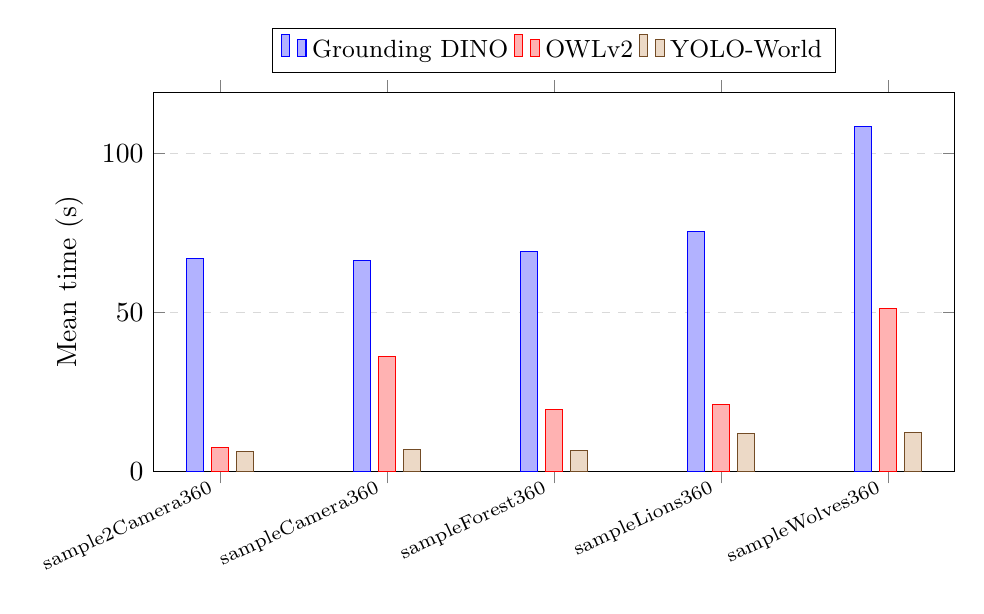
\begin{tikzpicture}
            \begin{axis}[
                ybar=3pt,
                bar width=6pt,
                width=0.97\textwidth,
                height=6.4cm,
                ymin=0,
                ylabel={Mean time (s)},
                symbolic x coords={v1,v2,v3,v4,v5},
                xtick=data,
                xticklabels={sample2Camera360,sampleCamera360,sampleForest360,sampleLions360,sampleWolves360},
                x tick label style={rotate=25,anchor=east,font=\scriptsize},
                legend style={font=\small,at={(0.5,1.05)},anchor=south,legend columns=3},
                ymajorgrids=true,
                grid style={dashed,gray!30}
            ]
                \addplot coordinates {(v1,66.81) (v2,66.18) (v3,69.17) (v4,75.45) (v5,108.31)};
                \addplot coordinates {(v1,7.50) (v2,36.25) (v3,19.65) (v4,21.20) (v5,51.24)};
                \addplot coordinates {(v1,6.43) (v2,6.99) (v3,6.65) (v4,12.01) (v5,12.21)};
                \legend{Grounding DINO, OWLv2, YOLO-World}
            \end{axis}
        \end{tikzpicture}
        \caption{Mean inference time per video.}
    \end{subfigure}

    \vspace{0.8em}

    \begin{subfigure}{\textwidth}
        \centering
        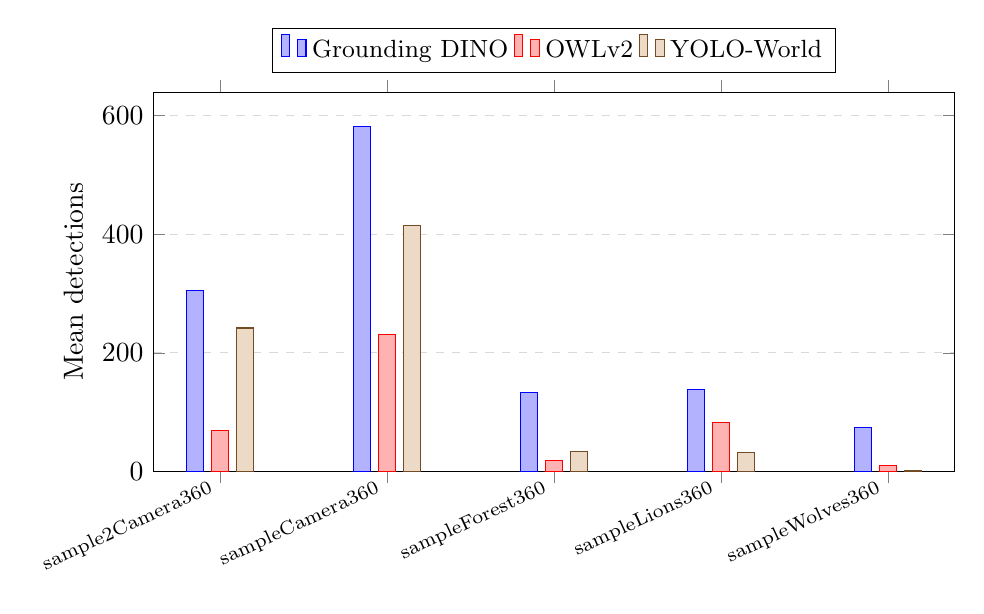
\begin{tikzpicture}
            \begin{axis}[
                ybar=3pt,
                bar width=6pt,
                width=0.97\textwidth,
                height=6.4cm,
                ymin=0,
                ylabel={Mean detections},
                symbolic x coords={v1,v2,v3,v4,v5},
                xtick=data,
                xticklabels={sample2Camera360,sampleCamera360,sampleForest360,sampleLions360,sampleWolves360},
                x tick label style={rotate=25,anchor=east,font=\scriptsize},
                legend style={font=\small,at={(0.5,1.05)},anchor=south,legend columns=3},
                ymajorgrids=true,
                grid style={dashed,gray!30}
            ]
                \addplot coordinates {(v1,305) (v2,581) (v3,133) (v4,138) (v5,74)};
                \addplot coordinates {(v1,69) (v2,231) (v3,18) (v4,83) (v5,10)};
                \addplot coordinates {(v1,242) (v2,414) (v3,34) (v4,32) (v5,2)};
                \legend{Grounding DINO, OWLv2, YOLO-World}
            \end{axis}
        \end{tikzpicture}
        \caption{Mean number of exported detections per video.}
    \end{subfigure}
    \caption{Detector benchmark on the five-video engineering benchmark set with per-video semantic prompts. The upper chart shows the runtime trade-off among the three detectors, whereas the lower chart shows the corresponding detection yield after adapting the prompt vocabulary to each stimulus.}
    \label{fig:detector-benchmark}
\end{figure}

From the standpoint of this project, the benchmark leads to three practical conclusions. First, the detector stage should remain configurable rather than hard-coded, because the ``best'' model depends not only on speed versus coverage, but also on how well the prompt vocabulary fits the stimulus. Second, YOLO-World is the most useful exploratory backend in this benchmark: it is consistently the fastest option and performs strongly on the human- and device-centric clips. Third, Grounding DINO is the safest choice when difficult scenes require robust coverage before the AOI sequence is frozen, whereas OWLv2 should be treated as a viable experimental alternative whose main value lies between the other two models. For that reason, the benchmark reported here is best understood as an engineering filter for the preprocessing stage, not as a substitute for later validation against manual annotations and downstream gaze metrics.

The target version of the method extends this pipeline in three ways. First, detection boxes will be refined into masks through a segmentation stage, rather than remaining box-like approximations. Second, temporal propagation and re-detection will be strengthened to better handle appearance changes, occlusion, and discontinuous motion. Third, human validation will be added as an explicit quality-control stage in which AOI outputs can be reviewed and corrected before they are frozen as experimental inputs. This staged roadmap keeps the current implementation useful for integration while preserving a clear path toward the full methodological study.


\subsection{Logging and synchronisation}

The runtime logging layer was designed to prioritise auditability, deterministic stimulus alignment, and downstream reproducibility. In line with the architectural assumptions of the system, gaze data were not treated as screen-space samples but as observations mapped to the spherical coordinate system of the 360\textdegree\ stimulus. Accordingly, each gaze sample was associated with the frame actually displayed by the video player, rather than relying exclusively on continuous timestamps.

To avoid conflating raw instrumentation with derived analytical outputs, the data model was split into distinct artefacts. First, a raw sample log stores frame-synchronised gaze observations, including session metadata, timestamp information, head- or device-space origin and direction vectors, spherical coordinates, UV coordinates, AOI assignment, AOI confidence, pupil-related measures, and validity flags. Second, a fixation-event log stores higher-level events derived from the raw stream through a reproducible fixation detection procedure. Third, a session-level summary file records calibration status, exclusion criteria, data-quality indicators, and runtime incidents. This separation ensures that analytical decisions remain inspectable and that downstream metrics can be recomputed if fixation parameters or AOI assignment rules change.

The raw sample log constitutes the canonical source for subsequent processing. At minimum, each record should include: participant identifier, session identifier, stimulus identifier, monotonic timestamp, displayed frame index, gaze origin, gaze direction, azimuth, elevation, UV coordinates, AOI identifier, AOI confidence, left and right pupil diameter, and sample-validity status. Additional fields may include eye-specific validity, tracking source, calibration state, and head pose variables when required by the study design.

This design was adopted for three reasons. First, frame-level synchronisation reduces ambiguity when decoded video frames are presented with non-uniform timing. Second, storing gaze in spherical stimulus coordinates establishes a common reference space for gaze, AOIs, and later analyses. Third, separating raw samples from fixation-level outputs avoids irreversible preprocessing decisions at acquisition time and improves reproducibility.

For the present project, only fields that support experimental traceability or downstream analysis are considered mandatory. Interface-only variables, redundant transforms, and debug overlays are treated as optional and should not be allowed to destabilise the schema. Likewise, AOI assignment must be stored as the best available runtime lookup result, but the final methodological evaluation will determine whether the automatic AOI pipeline preserves gaze-based metrics relative to manual AOIs.

In the current prototype, CSV export is fixation-based rather than raw-sample-complete: the runtime commits fixation events every 250 ms and writes AOI-linked rows at that cadence. This choice was made to validate the end-to-end integration path early while keeping runtime logging volume manageable during device-side testing. Whenever the runtime can resolve the repository root, these CSV files are written directly into the repository \texttt{data/exports} folder so that the post-processing stage can consume them without an additional manual copy step. The broader analytical design, however, still assumes a future separation between raw gaze samples and derived fixation events when the final experimental protocol is frozen.

\subsubsection{Runtime data artefacts}

The runtime layer should produce, at minimum, the following files:

\begin{itemize}
    \item \texttt{raw\_gaze\_samples.csv}: canonical frame-synchronised gaze data.
    \item \texttt{fixation\_events.csv}: derived fixation-level events computed from the raw sample stream.
    \item \texttt{session\_summary.csv}: per-session calibration, validity, exclusion, and quality-control summary.
    \item \texttt{runtime\_incidents.csv}: optional log of tracking loss, recalibration, dropped frames, or operator notes.
\end{itemize}

\subsubsection{Mandatory fields in \texttt{raw\_gaze\_samples.csv}}

The following fields are proposed as mandatory in the raw gaze log:

\begin{itemize}
    \item \texttt{participant\_id}
    \item \texttt{session\_id}
    \item \texttt{video\_id}
    \item \texttt{timestamp\_ms}
    \item \texttt{frame\_index}
    \item \texttt{origin\_x}, \texttt{origin\_y}, \texttt{origin\_z}
    \item \texttt{direction\_x}, \texttt{direction\_y}, \texttt{direction\_z}
    \item \texttt{azimuth\_rad}
    \item \texttt{elevation\_rad}
    \item \texttt{uv\_x}, \texttt{uv\_y}
    \item \texttt{aoi\_id}
    \item \texttt{aoi\_confidence}
    \item \texttt{left\_pupil\_diameter}
    \item \texttt{right\_pupil\_diameter}
    \item \texttt{is\_valid}
\end{itemize}

\subsubsection{Recommended fields to add in the next iteration}

To strengthen experimental traceability, the following fields are recommended for the next implementation iteration:

\begin{itemize}
    \item \texttt{tracking\_source}
    \item \texttt{left\_eye\_valid}, \texttt{right\_eye\_valid}
    \item \texttt{calibration\_state}
    \item \texttt{head\_pos\_x}, \texttt{head\_pos\_y}, \texttt{head\_pos\_z}
    \item \texttt{head\_rot\_qx}, \texttt{head\_rot\_qy}, \texttt{head\_rot\_qz}, \texttt{head\_rot\_qw}
    \item \texttt{video\_time\_ms}
    \item \texttt{sample\_index}
\end{itemize}

\subsubsection{Fields that should not be treated as part of the stable core schema}

The following categories should remain outside the stable core schema unless they become necessary for a specific analysis:

\begin{itemize}
    \item transient debug variables used only for visual overlays,
    \item duplicated coordinate representations with no analytical value,
    \item intermediate AOI lookup diagnostics that can be regenerated offline,
    \item model-internal variables from the offline AOI generation stage.
\end{itemize}



\subsection{Ground-truth manual annotations}

A manually annotated reference set is required in order to evaluate whether automatically generated dynamic AOIs remain valid for downstream gaze analysis. In this project, manual annotations are not treated as an informal visual check, but as a methodological baseline against which the automatic pipeline can be compared both spatially and in terms of derived eye-tracking metrics.

The architecture of the system assumes that dynamic AOIs are generated offline and later consumed at runtime as masks or ID maps. This design makes manual annotation especially important for two reasons. First, it provides a defensible reference against which automatic AOIs can be evaluated. Second, it enables the study to distinguish between errors introduced by the AOI-generation pipeline and errors introduced by the gaze-acquisition or synchronisation layers.

The manual reference set should therefore be constructed as a bounded but high-quality corpus rather than as exhaustive annotation of all available stimuli. For the first validation stage, the recommended design is to annotate a small set of short 360\textdegree\ videos containing both standard and difficult conditions, including seam crossings, small objects, temporal drift, and occlusions. Each video should include a predefined inventory of AOIs with stable semantic labels and explicit rules for appearance, disappearance, overlap, and object splitting at the equirectangular seam.

Manual annotations should be represented as masks or per-frame ID maps rather than bounding boxes alone. Bounding boxes may be retained as debugging aids, but they should not constitute the final reference representation when AOIs are irregular, small, or located near the left-right seam of the equirectangular frame. For the same reason, annotation rules should explicitly state how to treat partially visible objects, ambiguous boundaries, and merged or split instances across time.

To improve methodological defensibility, the annotation process should be documented through a written protocol and should include, at least on a subset of the corpus, double annotation by two human annotators. The purpose of this step is not to assume that manual labels are error-free, but to quantify the stability of the reference definition itself. Any AOI class or scene type that yields low inter-annotator agreement should be revised before it is used as a baseline in the main validation.

The manual ground-truth package should contain four components: (1) the annotated masks or ID maps, (2) metadata linking each annotation to participant-independent video and frame information, (3) an AOI ontology with semantic labels and inclusion/exclusion rules, and (4) annotation logs describing edge cases, corrections, and unresolved ambiguities. This package should be versioned and frozen before the main comparison with the automatic AOI pipeline.

The primary role of the manual reference set in the paper will be twofold. First, it will support spatial comparison using agreement measures such as IoU and Dice. Second, and more importantly, it will support downstream validation by quantifying the extent to which AOI source (manual versus automatic) affects metrics such as time to first fixation, fixation duration, total fixation duration, fixation count, and fixation order. In this sense, the manual annotation stage is not merely preparatory; it is one of the central methodological pillars of the study.

\subsubsection{Minimum requirements for the manual reference set}

The manual reference set should satisfy the following minimum conditions:

\begin{itemize}
    \item inclusion of both easy and difficult 360\textdegree\ scenes,
    \item explicit AOI definitions before annotation begins,
    \item per-frame masks or ID maps as the preferred final representation,
    \item documented rules for seam crossings, partial visibility, and temporal continuity,
    \item double annotation on a subset of the material,
    \item versioned release prior to automatic-versus-manual comparison.
\end{itemize}

\subsubsection{Recommended annotation outputs}

The following artefacts are recommended:

\begin{itemize}
    \item \texttt{manual\_gt/} with masks or ID maps per frame,
    \item \texttt{aoi\_ontology.csv} with AOI labels and definitions,
    \item \texttt{annotation\_decisions.md} with edge-case resolutions,
    \item \texttt{inter\_annotator\_agreement.csv} for the doubly annotated subset.
\end{itemize}


\subsection{Validation design}
The validation framework includes:
\begin{itemize}[leftmargin=1.5em]
    \item technical validation of the runtime and gaze logging,
    \item spatial validation of automatic AOIs against manual AOIs,
    \item downstream validation of gaze-based metrics computed from both AOI sources.
\end{itemize}

\section{Results}

\subsection{Technical validation}
At the present implementation stage, the main technical result is the availability of a stable end-to-end prototype rather than a final numerical benchmark. The runtime now supports panoramic video playback, OpenXR eye-gaze acquisition with HTC fallback, spherical gaze mapping, exact-color AOI lookup, AOI sequence loading by displayed frame index, loop-safe AOI reset, pupil-diameter capture when the device exposes that information, and fixation-based CSV export.

Several engineering adjustments were necessary to reach this stable state. AOI overlays were moved to a dedicated transparent sphere, yaw alignment was baked offline into exported AOI maps, and the runtime AOI sequence path was optimised through a binary RGB24 pack, reusable textures, preloading of the next keyframe, and lighter AOI-map resolutions for standalone playback. In addition, AOI confidence computation and overlay updates were trimmed to reduce unnecessary per-frame work. Quantitative profiling of valid sample rate, end-to-end latency, and dropped-frame behaviour remains part of the next validation stage.

\subsection{Spatial validation of AOIs}
Spatial validation against manual ground truth has not yet been completed, because the manual reference set is still being formalised. Nevertheless, the current automatic pipeline already produces the representation required for such evaluation: persistent AOI identities, exact-color AOI maps, and per-keyframe metadata indexed by absolute source-frame number. This means that frame-level comparisons such as IoU and Dice can be carried out once manual masks or ID maps are frozen.

From a systems perspective, the current spatial result is therefore preparatory but important: the automatic AOI representation is now stable enough to support a one-to-one comparison with manual annotations on the same frames. The next experimental milestone is to construct a manually annotated subset including seam crossings, distortion-heavy regions, and small or unstable targets so that the current representation can be stress-tested under the most informative 360\textdegree\ failure modes.

\subsection{Downstream gaze-metric validation}
Downstream validation is likewise not yet complete in quantitative terms, but the infrastructure required for it is now in place. The runtime exports fixation-linked records containing participant and session identifiers, frame index, world-space gaze origin and direction, spherical angles, UV coordinates, AOI identifier, AOI confidence, pupil diameters when available, and a validity flag. This schema is sufficient to compute TFF, FD, TFD, FC, and fixation-order comparisons once the manual and automatic AOI sources are applied to the same sessions.

The current post-processing stage already extends this contract with reproducible quality-control and aggregation outputs. In particular, the analytics pipeline now estimates fixation cadence per session, flags short or low-quality runs, summarizes source CSV files at ingestion time, and computes normalized AOI metrics such as dwell-time share, visit rate, and relative time to first fixation. It also aggregates engagement at the video-AOI level, which is the most direct bridge toward the planned manual-versus-automatic comparison.

In addition, the present implementation now includes an explicit comparison path in which the same fixation-linked Unity export can be re-evaluated against two different AOI-manifest roots, for example a manual reference package and an automatically generated package. Rather than requiring a second runtime recording, the comparison layer reuses the exported `video\_id`, `frame\_index`, and spherical UV coordinates, resolves AOI membership offline for both sources, and then emits session-alignment summaries, confusion tables, and per-video metric deltas. This makes the downstream validation design operational even before the final manual corpus is frozen, because the analytical contract no longer depends on Unity as the comparison engine.

Accordingly, the current result of this phase is not only the establishment of a reproducible analysis contract, but also the first operational version of the downstream analysis layer. The essential scientific question nevertheless remains open and will be answered in the next phase: whether substituting manually annotated AOIs with automatically generated AOIs materially changes the interpretation of gaze behaviour.

\subsection{Annotation effort reduction}
Even without a formal time-and-motion study, the present implementation already clarifies where annotation effort is likely to be reduced. The offline pipeline automates sparse frame extraction, proposal generation, AOI identity persistence across keyframes, AOI-map export, metadata export, and runtime-pack generation. In practice, this replaces a large portion of repetitive frame-by-frame redraw work with prompt design, threshold tuning, and targeted human review.

At the same time, the current system should not yet be described as fully automatic annotation. Human supervision remains necessary when detections are semantically wrong, when objects are unstable across keyframes, or when seam-aware reasoning is required. A formal comparison between manual annotation time and automatic-plus-review time remains a required part of the final study design.

\section{Discussion}

The main question is not whether automatic AOIs visually resemble manual AOIs, but whether they remain valid for downstream eye-tracking analysis. This distinction is central in immersive and dynamic stimuli, where even moderate spatial discrepancies may or may not translate into meaningful differences in gaze-based metrics.

The current implementation supports the central architectural claim of the project: separating offline AOI generation from runtime experimental execution is a sensible design choice for immersive eye-tracking studies. In practice, this separation simplified debugging, reduced the amount of model-dependent logic inside the headset runtime, and made it possible to optimise the experiment path around deterministic frame display, spherical mapping, and lightweight AOI lookup.

Several practical lessons emerged from the implementation. First, exact-color AOI contracts are far more scalable than ad hoc color heuristics when persistent object identities must be maintained across time. Second, in standalone VR, apparently minor runtime choices such as decoding per-frame PNGs, rebuilding overlays in CPU loops, or recalculating expensive confidence terms every frame can materially affect the smoothness of stimulus presentation. Third, alignment issues in 360\textdegree\ systems are often easier to solve in the preprocessing stage than in the real-time stage; baking a stable yaw offset offline proved cleaner than compensating dynamically in multiple runtime subsystems.

At the same time, the 360\textdegree\ domain continues to impose distinctive risks. Seam crossings can split a single semantic object into disconnected image regions. Distortion near poles makes small AOIs harder to detect and validate consistently. Sparse keyframes may be sufficient for some objects but not for rapid motion or strong occlusion. These factors reinforce the importance of evaluating not only spatial similarity but also downstream metric stability.

Practically, the system now appears mature enough to support the next methodological phase: freezing a manual reference subset, running comparative analyses, and identifying where automatic AOIs remain trustworthy and where manual intervention is still indispensable.

\section{Limitations}

Several limitations should be acknowledged. First, the current implementation has been validated primarily as an engineering and integration pipeline on a pilot stimulus rather than as a completed experimental corpus. Generalisability across content types, participant populations, and AOI ontologies therefore remains to be demonstrated.

Second, the current automatic AOI stage is still based on detection-derived regions rather than full segmentation masks. Although the architecture is compatible with segmentation and temporal propagation, the present AOIs should be understood as a first operational approximation, not the final representation.

Third, the system inherits limitations from equirectangular representation itself. Distortion varies across latitude, and seam handling remains a special case that must be treated explicitly in both annotation and validation. These are not merely implementation details; they are part of the measurement problem.

Fourth, the current runtime prototype writes fixation-based CSV output every 250 ms for integration purposes rather than a definitive high-frequency raw sample log. This is useful for validating the end-to-end path, but the final experimental protocol may require a richer raw stream for some analyses.

Finally, the current device-side validation has been centred on one hardware family and one runtime configuration. Broader validation across headsets, firmware revisions, and tracking conditions would strengthen the external validity of the proposed framework.

\section{Conclusion}

This work presents a methodological pipeline for the offline generation of dynamic AOIs in 360\textdegree\ video with VR eye tracking. The implemented system now provides a complete integration path from sparse frame extraction and automatic AOI authoring in Python to deterministic AOI playback, gaze mapping, and fixation-based logging in Unity. Its main scientific contribution, however, is not the software stack by itself, but the validation framework it enables: a comparison of automatic and manual AOIs both spatially and through downstream gaze-based metrics.

The current stage establishes the experimental substrate required for that comparison. The next stage is to complete the manual reference corpus, run the spatial and downstream validation analyses, and quantify annotation-effort reduction under realistic 360\textdegree\ conditions. If successful, the resulting framework could provide a reproducible and scalable route to immersive gaze analysis with substantially lower manual annotation cost.

\bibliographystyle{plain}
\bibliography{bibliografia}


\end{document}
